\section{最大质因数}
\subsection{问题描述}
\begin{tcolorbox}
	$13195$ 的质因数是 $5, 7, 13$ 和 $29$。

	求数 $600851475143$ 的最大质因数。

	\href{https://projecteuler.net/problem=3}{原题链接}
\end{tcolorbox}

\subsection{算法}
素数的判定是一个经典的算法问题,主要有以下一些常见的算法。这些算法根据使用场景的不同各有优劣。
\subsubsection{试除法}
\begin{algorithm}
	\caption{素数判断}
	\label{IsPrime}
	\begin{algorithmic}[1]
		\Function{IsPrime}{n}
		\State \( r \gets 2 \)
		\While{ \(  r \leqslant \lfloor \sqrt{n} \rfloor \)}
		\If{ \( n \bmod r = 0 \)}
		\Return false
		\EndIf
		\State \( r \gets r + 1 \)
		\EndWhile
		\Return true
		\EndFunction
	\end{algorithmic}
\end{algorithm}
这个素数判定法也称为试除法,已经比素数的定义做了一点优化。素数的定义是除了能被1和本身整除,这里只试除到 \(
\lfloor\sqrt{n}\rfloor \)。因为如果存在比 \( \lfloor\sqrt{n}\rfloor \)大的因子 \( i \),那么肯定也存在比个小于 \( \lfloor
\sqrt{n} \rfloor \)的因子 \( j \), 使得 \( i \times j = n \),而 \( j \)在之前已经判断过所以	\( i \)就不需要判断了。

\subsubsection{改进试除法}
试除法还可以进一步优化,主要有两点:
\begin{enumerate}
	\item 跳过偶数: 除了2以外,所有的素数都是奇数;
	\item 跳过合数:进一步跳过所有能够被2或者3整除的数,检查从5开始,每次递增6(即检查 \( 6k-1 \text{和} 6k + 1 \))。
\end{enumerate}
\begin{figure}[htbp]
	\centering
	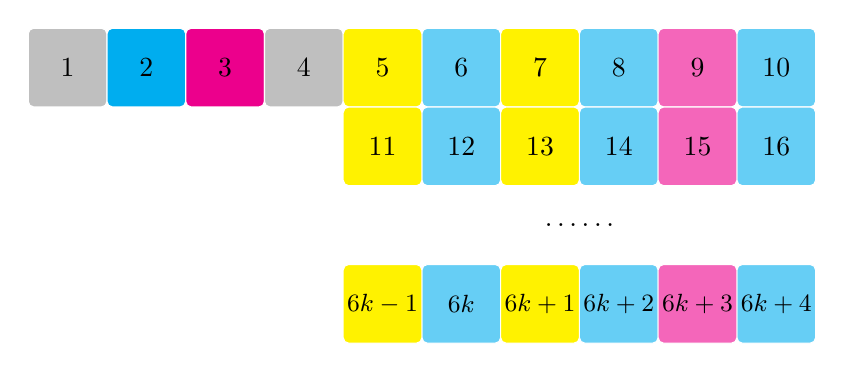
\begin{tikzpicture}[draw=white, rounded corners=2pt]
		\draw[fill=lightgray] (1,0) rectangle node{1}+(1,1);
		\draw[fill=cyan] (2,0) rectangle node{2}+(1,1);
		\draw[fill=magenta] (3,0) rectangle node{3}+(1,1);
		\draw[fill=lightgray] (4,0) rectangle node{4}+(1,1);
		\foreach \x in {6,8,10}
			{
				\draw[fill=cyan!60] (\x, 0) rectangle node{\x} +(1,1) ;
			}
		\draw[fill=yellow] (5,0) rectangle node{5}+(1,1);
		\draw[fill=yellow] (7,0) rectangle node{7}+(1,1);
		\draw[fill=magenta!60] (9,0) rectangle node{9} +(1,1);
		\foreach \x in {6,8,10}
			{
				\draw[fill=cyan!60] (\x, -1) rectangle
				node{\pgfmathparse{int(\x + 6)}\pgfmathresult} +(1,1) ;
			}
		\draw[fill=yellow] (5,-1) rectangle node{11}+(1,1);
		\draw[fill=yellow] (7,-1) rectangle node{13}+(1,1);
		\draw[fill=magenta!60] (9,-1) rectangle node{15} +(1,1);
		\node at (8, -1.5) {$\dots\dots$};
		\foreach \x/\n in {6/$6k$,8/$6k+2$,10/$6k+4$}
			{
				\draw[fill=cyan!60] (\x, -3) rectangle
				node{\small\n} +(1,1) ;
			}
		\draw[fill=yellow] (5,-3) rectangle node{\small$6k-1$}+(1,1);
		\draw[fill=yellow] (7,-3) rectangle node{\small$6k+1$}+(1,1);
		\draw[fill=magenta!60] (9,-3) rectangle node{\small$6k+3$} +(1,1);
	\end{tikzpicture}
	\caption{试除法改进图示}
\end{figure}

\begin{algorithm}[htbp]
	\caption{改进的素数判断}
	\label{algo:IsPrimeImproved}
	\begin{algorithmic}[1]
		\Function{IsPrimeImproved}{n}
		\If{ \( n \leqslant 3 \)}
		\Return \( n > 1 \)
		\EndIf
		\If{ \( n \bmod 2 = 0 \textbf{ or } n \bmod 3 = 0 \)}
		\Return false
		\EndIf
		\State \( r \gets 5 \)
		\While{ \( r^2 \leqslant n \)}
		\If{ \( n \bmod r = 0 \textbf{ or } n \bmod (r + 2) = 0 \)}
		\Return false
		\EndIf
		\State \( r \gets r + 6 \)
		\EndWhile
		\Return true
		\EndFunction
	\end{algorithmic}
\end{algorithm}
这种算法效率比普通的试除法高得多,尤其是当 \( n \) 很大时。

\subsubsection{埃拉托斯特尼筛法}
如果需要判断多个数是否为素数,可以预先生成素数表。这种算法是通过逐步标记合数的方式生成所有不大于某个给定数 \( N \) 的素数表。伪代码如下:
\begin{algorithm}
	\caption{埃拉托斯特尼筛法}
	\label{algo:SieveOfEratosthenes}
	\begin{algorithmic}[1]
		\Function{SieveOfEratosthenes}{N}
		\State 创建布尔数组 \textit{primes},大小为 \( N+1 \),初始全为 \textbf{true}
		\State \( \textit{primes}[0] \gets \textbf{false} \)
		\State \( \textit{primes}[1] \gets \textbf{false} \) \Comment{0 和 1 不是素数}
		\For{ \( p \gets 2 \) \textbf{to} \( \lfloor \sqrt{N} \rfloor \)}
		\If{ \( primes[p] = \textbf{true} \)}
		\For{ \( i \gets p^2 \) to \( N \) by \( p \)}
		\State \( \textit{primes}[i] \gets \textbf{false} \)
		\EndFor
		\EndIf
		\EndFor
		\Return \textit{primes}
		\EndFunction
	\end{algorithmic}
\end{algorithm}

可以看到这种筛法里面有重复的计算,比如8会被4和2都筛一次,如果数值较大的情况下,算力浪费较多。

\subsubsection{欧拉筛法}
欧拉筛法是对埃拉托斯特尼筛法的改进,去除重复筛选的部分。欧拉筛法的关键是每个合数只被最小质因数筛选一次。
伪代码如下:
\begin{algorithm}
	\caption{欧拉筛法}
	\label{algo:SieveOfEuler}
	\begin{algorithmic}[1]
		\Function{SieveOfEuler}{N}
		\State 创建布尔数组 \textit{primeStatus},大小为 \( N+1 \),初始全为 \textbf{true}
		\State \( \textit{primeStatus}[0] \gets \textbf{false} \)
		\State \( \textit{primeStatus}[1] \gets \textbf{false} \) \Comment{0 和 1 不是素数}
		\State 创建数组 \textit{primes}用于存放素数,初始为空
		\For{ \( n \gets 2 \) to \( \lfloor \sqrt{N} \rfloor + 1 \)}
		\If{ \( primeStatus[n] = \textbf{true} \)}
		\State 将 n 推进 primes 数组中
		\EndIf
		\For{每个 \( primes \)中的素数 \( p \)}
		\If{ n \times p > n} \State break \Comment{越界检查}
		\EndIf
		\State \(  {primeStatus[n \times p] \gets \textbf{false}}\)
		\If{ \( p \mid n\)} \Comment{这一步是关键,如果p整除n,则中止循环。比如循环到 \( n=15
		\)时,首先会将30标记为合数,然后是45,但是因为3整除15,所以就中止循环。这样就使得后面的60这些数只被它的最小质因数筛一次。}
		\State break;
		\EndIf
		\EndFor
		\EndFor
		\Return \textit{primes}
		\EndFunction
	\end{algorithmic}
\end{algorithm}

\subsubsection{米勒-拉宾素性测试}
\subsubsection*{米勒-拉宾素性测试的原理}
\begin{enumerate}
	\item 基本概念

	      米勒-拉宾测试是基于以下数学定理:

	      费马小定理(Fermat's Little Theorem):
	      如果 \( p \) 是素数,且 \( a \) 是任意整数且 \( a \) 不被 \( p \) 整除,那么:
	      \[ a^{p-1} \equiv 1 \pmod{p} \]

	      米勒-拉宾测试通过对这个定理进行扩展,来检查一个数是否可能是素数。它是一个概率性算法,意味着测试结果可能存在一定的误差,但通过多次测试,可以使误差变得非常小。
	\item  算法步骤

	      以下是米勒-拉宾素性测试的基本步骤:

	      \begin{enumerate}
		      \item	输入处理:

		            输入一个待测试的正整数 \( n \) 和测试轮数 \( k \)。轮数 \( k \) 是一个用于提高算法准确性的参数。
		      \item	特殊情况处理:

		            \begin{itemize}
			            \item	如果 \( n \leqslant 1 \),则 \( n \) 不是素数。
			            \item	如果 \( n \) 是偶数且大于 2,则 \( n \) 不是素数。
			            \item	如果 \( n \) 是 2 或 3,则 \( n \) 是素数。
		            \end{itemize}
		      \item	将 \( n-1 \) 表示为 \( d \times 2^r \):

		            将 \( n-1 \) 表示为 \( d \times 2^r \),其中 \( d \) 是奇数,\( r \) 是非负整数。
		      \item	进行 \( k \) 轮测试:
		            对于每一轮测试:
		            \begin{itemize}
			            \item	随机选择一个整数 \( a \)(\( 2 \leqslant a \leqslant n-2 \))。
			            \item	计算 \( x = a^d \mod n \)。
			            \item	如果 \( x \) 等于 1 或 \( n-1 \),则继续到下一轮测试。
			            \item	如果 \( x \) 不等于 1 和 \( n-1 \),则进行以下检查:
			            \item	对 \( r-1 \) 次迭代,每次计算 \( x = x^2 \mod n \)。
			            \item	如果在任何一次迭代中 \( x \) 等于 \( n-1 \),则继续到下一轮测试。
			            \item	如果所有 \( r-1 \) 次迭代都没有找到 \( x \) 等于 \( n-1 \),则 \( n \) 被认为是合数,返回 false。
		            \end{itemize}
		      \item	结果:
		            \begin{itemize}
			            \item	如果在所有 \( k \) 轮测试中,\( n \) 没有被发现是合数,则返回 true,表示 \( n \) 是素数。
		            \end{itemize}
	      \end{enumerate}
	\item 数学依据

	      米勒-拉宾测试依赖于以下定理和结果:

	      米勒定理:
	      如果一个数 \( n \) 不是素数,那么存在一个值 \( a \) 使得:
	      \[ a^d \not\equiv 1 \pmod{n} \text{ 且 } a^{2^i \cdot d} \not\equiv n-1 \pmod{n} \]
	      对于所有 \( i \) 从 \( 0 \) 到 \( r-1 \)。

	      这个定理提供了一个检查合数的有效方法:如果一个数在测试中未能满足这些条件,那么它很可能是合数。
	\item 概率性

	      •	米勒-拉宾测试是概率性的,这意味着它不能绝对确定一个数是否是素数,但可以通过多轮测试将错误率降低到很小的水平。每次测试失败的概率是非常小的,因此可以通过增加测试轮数来提高准确性。

	      米勒-拉宾测试的时间复杂度是 \( O(k \cdot \log^3 n) \),其中 \( k \) 是测试轮数,\( \log n \) 是  n  的位数。这个复杂度使得米勒-拉宾测试非常适合用于大数的素数测试。
\end{enumerate}

\begin{algorithm}
	\caption{米勒-拉宾素性测试}
	\begin{algorithmic}[1]
		\Function{MillerRabin}{n, k} \Comment{k 是测试的轮数}
		\If{ \( n \leqslant 2 \)}
		\Return false
		\EndIf
		\If{ \( n \bmod 2 = 0 \)}
		\Return false
		\EndIf
		\State 将 \( n - 1 \) 表示为 \( d \times 2^r \),其中 \( d \) 是奇数
		\For{ \( i \gets 1 \) to \( k \)}
		\State 随机选择整数 \( a \) ,使得 \( 2 \leqslant a \leqslant n-2 \)
		\State \( x \gets a^d \bmod n \)
		\If{ \( x = 1 \text{ or } x = n-1 \)}
		\textbf{continue}
		\EndIf
		\For{ \( j \gets 1 \) to \( r-1 \)}
		\State \( x \gets x^2 \bmod n \)
		\If{ \( x = n-1 \)}
		\textbf{break}
		\EndIf
		\EndFor
		\If{ \( x \neq n-1 \)}
		\Return false
		\EndIf
		\EndFor
		\Return true
		\EndFunction
	\end{algorithmic}
\end{algorithm}

\begin{algorithm}
	\caption{最大质因数}
	\begin{algorithmic}[1]
		\Function{GreatestPrimeFactor}{n}
		\State \textbf{输入:} 数组 primes
		\For{ 每个在primes中的\( p \)}
		\While{ \( n \mod p = 0 \)}
		\State \( n \gets n \div p \)
		\EndWhile
		\If{ \( p \geqslant n \)}
		\State \textbf{break}
		\EndIf
		\EndFor
		\Return \( p \)
		\EndFunction
	\end{algorithmic}
\end{algorithm}
